\documentclass[tikz,border=10pt]{standalone}
\usepackage[utf8]{vietnam}
\usepackage{tgheros}
\usepackage{sansmath}
\sansmath
\renewcommand{\familydefault}{\sfdefault}
\begin{document}
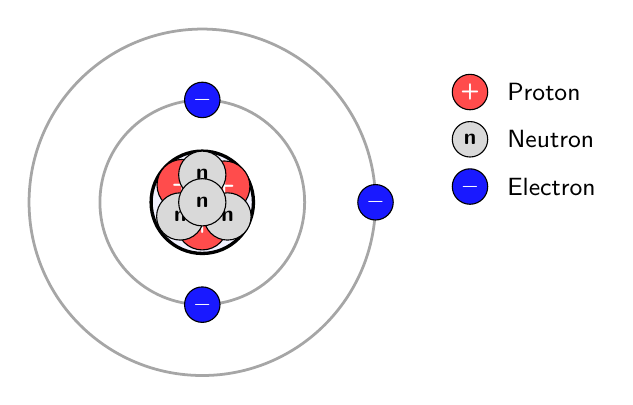
\begin{tikzpicture}[x=1cm, y=1cm, line cap=round, line join=round]
  % Định nghĩa bán kính
  \def\rK{1.3}
  \def\rL{2.2}
  \def\rNuc{0.65}

  % Vòng quỹ đạo electron
  \draw[line width=1.0pt, gray!70] (0,0) circle (\rK);
  \draw[line width=1.0pt, gray!70] (0,0) circle (\rL);

  % Hạt nhân (vòng viền)
  \draw[line width=1.2pt, fill=blue!5] (0,0) circle (\rNuc);

  % Các hạt trong hạt nhân: 3 proton (màu đỏ có dấu +), 4 neutron (màu xám nhạt)
  % Proton 1, 2, 3
  \node[circle, draw=black, fill=red!70, inner sep=0pt, minimum size=6.5mm, font=\bfseries\small, text=white] at (-0.25, 0.22) {+};
  \node[circle, draw=black, fill=red!70, inner sep=0pt, minimum size=6.5mm, font=\bfseries\small, text=white] at (0.28, 0.20) {+};
  \node[circle, draw=black, fill=red!70, inner sep=0pt, minimum size=6.5mm, font=\bfseries\small, text=white] at (0.0, -0.28) {+};

  % Neutron 1, 2, 3, 4
  \node[circle, draw=black, fill=gray!30, inner sep=0pt, minimum size=6.0mm, font=\bfseries\footnotesize] at (-0.28, -0.18) {n};
  \node[circle, draw=black, fill=gray!30, inner sep=0pt, minimum size=6.0mm, font=\bfseries\footnotesize] at (0.32, -0.18) {n};
  \node[circle, draw=black, fill=gray!30, inner sep=0pt, minimum size=6.0mm, font=\bfseries\footnotesize] at (0.0, 0.35) {n};
  \node[circle, draw=black, fill=gray!30, inner sep=0pt, minimum size=6.0mm, font=\bfseries\footnotesize] at (0.0, 0.0) {n};

  % Electron lớp 1 (K): 2 electron
  \node[circle, draw=black, fill=blue!90, inner sep=0pt, minimum size=4.5mm, font=\bfseries\footnotesize, text=white] at (0, \rK) {$-$};
  \node[circle, draw=black, fill=blue!90, inner sep=0pt, minimum size=4.5mm, font=\bfseries\footnotesize, text=white] at (0, -\rK) {$-$};

  % Electron lớp 2 (L): 1 electron
  \node[circle, draw=black, fill=blue!90, inner sep=0pt, minimum size=4.5mm, font=\bfseries\footnotesize, text=white] at (\rL, 0) {$-$};

  % Chú thích bên cạnh
  \begin{scope}[shift={(3.4, 0.8)}]
    \node[circle, draw=black, fill=red!70, inner sep=0pt, minimum size=4.5mm, font=\bfseries\footnotesize, text=white] at (0, 0.6) {+};
    \node[right, font=\small] at (0.35, 0.6) {Proton};

    \node[circle, draw=black, fill=gray!30, inner sep=0pt, minimum size=4.5mm, font=\bfseries\footnotesize] at (0, 0.0) {n};
    \node[right, font=\small] at (0.35, 0.0) {Neutron};

    \node[circle, draw=black, fill=blue!90, inner sep=0pt, minimum size=4.5mm, font=\bfseries\footnotesize, text=white] at (0, -0.6) {$-$};
    \node[right, font=\small] at (0.35, -0.6) {Electron};
  \end{scope}
\end{tikzpicture}
\end{document}
